% updated April 2002 by Antje Endemann
% Based on CVPR 07 and LNCS, with modifications by DAF, AZ and elle, 2008 and AA, 2010, and CC, 2011; TT, 2014; AAS, 2016; AAS, 2020

% \documentclass[runningheads]{llncs}
% \documentclass[arXiv_main.tex]{subfiles}
\documentclass[crop=false]{standalone}

\usepackage{graphicx}
% DO NOT USE \usepackage{times}, it will be removed by typesetters
%\usepackage{times}

\usepackage{tikz}
\usepackage{comment} 
\usepackage{amsmath,amssymb} % define this before the line numbering.
\usepackage{color}

\usepackage{graphicx}
\usepackage{multirow}
\usepackage{bm}
\usepackage{float}

% \definecolor{yang_olive}{rgb}{0.5,0.5,0} 
% \definecolor{del_gray}{rgb}{0.8,0.8,0.8} 
% \newcommand\pjl[1]{\textcolor{black}{#1}}
% \newcommand\peng[1]{\textcolor{black}{#1}}
% \newcommand\wca[1]{\textcolor{black}{#1}}
% \newcommand\wfb[1]{\textcolor{black}{#1}}
% \newcommand\deleted[1]{\textcolor{del_gray}{#1}}
% \newcommand\old[1]{\textcolor{yellow}{\textit{#1}}}
% \newcommand{\yang}[1]{\textcolor{black}{#1}}
% \newcommand{\rev}[1]{\textcolor{blue}{#1}}

% % \newcommand\CRpjl[1]{\textcolor{red}{#1}}
% % \newcommand\CRpeng[1]{\textcolor{black}{#1}}
% % \newcommand\CRwca[1]{\textcolor{pink}{#1}}
% % \newcommand\CRwfb[1]{\textcolor{blue}{#1}}
% % \newcommand{\CRyang}[1]{\textcolor{yang_olive}{#1}}

% \newcommand\CRpjl[1]{\textcolor{black}{#1}}
% \newcommand\CRpeng[1]{\textcolor{black}{#1}}
% \newcommand\CRwca[1]{\textcolor{black}{#1}}
% \newcommand\CRwfb[1]{\textcolor{black}{#1}}
% \newcommand{\CRyang}[1]{\textcolor{black}{#1}}


% INITIAL SUBMISSION - The following two lines are NOT commented
% CAMERA READY - Comment OUT the following two lines
%\usepackage{ruler}
%\usepackage[width=122mm,left=12mm,paperwidth=146mm,height=193mm,top=12mm,paperheight=217mm]{geometry}



\begin{document}
% \renewcommand\thelinenumber{\color[rgb]{0.2,0.5,0.8}\normalfont\sffamily\scriptsize\arabic{linenumber}\color[rgb]{0,0,0}}
% \renewcommand\makeLineNumber {\hss\thelinenumber\ \hspace{6mm} \rlap{\hskip\textwidth\ \hspace{6.5mm}\thelinenumber}}
% \linenumbers
\pagestyle{headings}
\mainmatter
\def\ECCVSubNumber{100}  % Insert your submission number here

\title{Chained-Tracker: Chaining Paired Attentive Regression Results for End-to-End Joint Multiple-Object Detection and Tracking (Supplementary Material)} % 


% INITIAL SUBMISSION 
\begin{comment}
\titlerunning{ECCV-20 submission ID \ECCVSubNumber} 
\authorrunning{ECCV-20 submission ID \ECCVSubNumber} 
\author{Anonymous ECCV submission}
\institute{Paper ID \ECCVSubNumber}
\end{comment}
%******************

% CAMERA READY SUBMISSION
%\begin{comment}
\titlerunning{Supplementary Material for ``Chained-Tracker''}
% If the paper title is too long for the running head, you can set
% an abbreviated paper title here
%
\author{Jinlong Peng\inst{1} $^\star$ \and
Changan Wang\inst{1}
\thanks{\textit{Equal contribution.}}
\and
Fangbin Wan\inst{2} \and
Yang Wu\inst{3} 
\thanks{\textit{Corresponding author: Yang Wu (wuyang0321@gmail.com)}}
\and
Yabiao Wang\inst{1} \and
Ying Tai\inst{1} \and
Chengjie Wang\inst{1} \and
Jilin Li\inst{1} \and
Feiyue Huang\inst{1} \and
Yanwei Fu\inst{2}
}

%
\authorrunning{J. Peng et al.}
% First names are abbreviated in the running head.
% If there are more than two authors, 'et al.' is used.
%
\institute{Tencent Youtu Lab \quad
\email{\{jeromepeng, changanwang, caseywang, yingtai, jasoncjwang, jerolinli, garyhuang\}@tencent.com}
\and Fudan University \quad
\email{\{fbwan18, yanweifu\}@fudan.edu.cn}
\and
Nara Institute of Science and Technology \quad
\email{yangwu@rsc.naist.jp}
}
%\end{comment}
%******************
\maketitle

\section{Overview}

This supplementary material includes:

\noindent(1) The detailed design of the CTracker network architecture. (Sec. \ref{section:s_network})

\noindent(2) The details of data augmentation in training. (Sec. \ref{subsection:s_aug})

\noindent(3) The details of Chained-Anchors setting. (Sec. \ref{subsection:s_anchor})

\noindent(4) The detailed experiment results of CTracker and the qualitative comparison with other SOTA methods, including POI \cite{yu2016poi} and Tracktor \cite{bergmann2019tracking}. (Sec. \ref{section:s_exp})

\noindent(5) The experiment of adding the appearance feature to CTracker. (Sec. \ref{section:s_feature})

\section{Details of Network Architecture\label{section:s_network}}

As in Fig. \ref{fig:backbone}, we refer to Resnet50 \cite{he2016deep} and FPN \cite{lin2017feature} to build multi-scale feature representations at five scale levels, we denote them as $\{P_2, P_3, P_4, P_5, P_6\}$.

\begin{figure*}[ht]
\vspace{-5mm}
\centering{}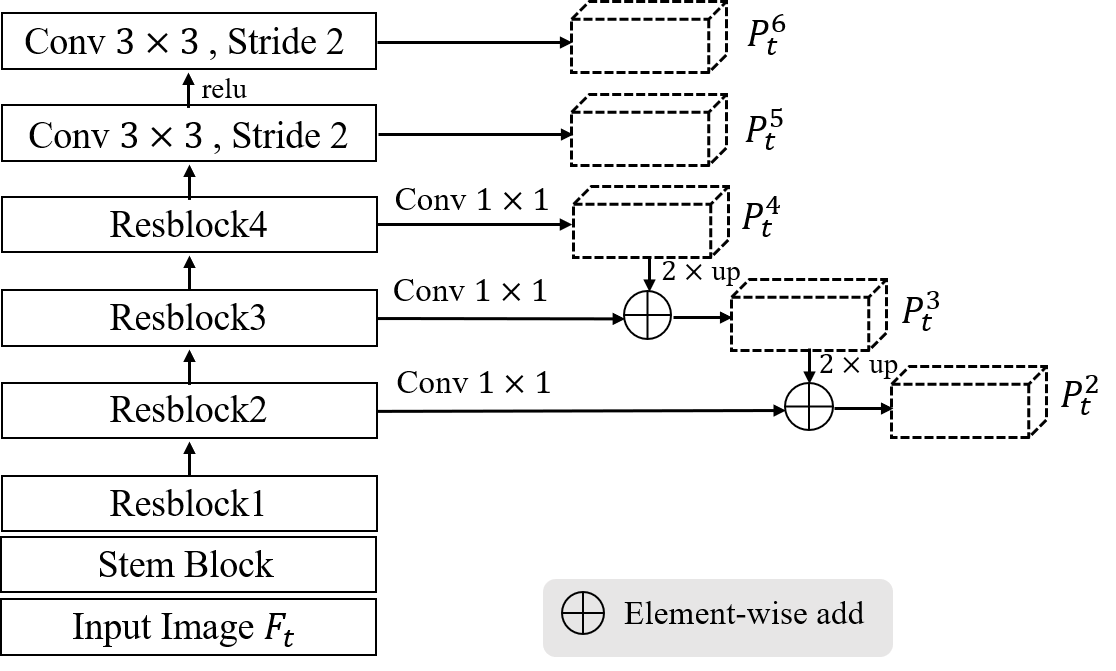
\includegraphics[width=0.54\columnwidth]{figure/figure2.png}
\vspace{-5mm}
\caption{\label{fig:backbone}\textbf{The detailed architecture of backbone in CTracker network.}}
\vspace{-3mm}
\end{figure*}

Then we combine the features from two adjacent frames at each scale for subsequent prediction, as in Fig. \ref{fig:head},. With the combined features, we apply two parallel branches to perform object classification and ID verification. The two branches consist of four consecutive 3$\times$3 conv layers interleaved with ReLU activations to perform feature learning for specific tasks, above which a 3$\times$3 conv with Sigmoid activation is appended to predict the confidence.  

\begin{figure*}[ht]
\centering{}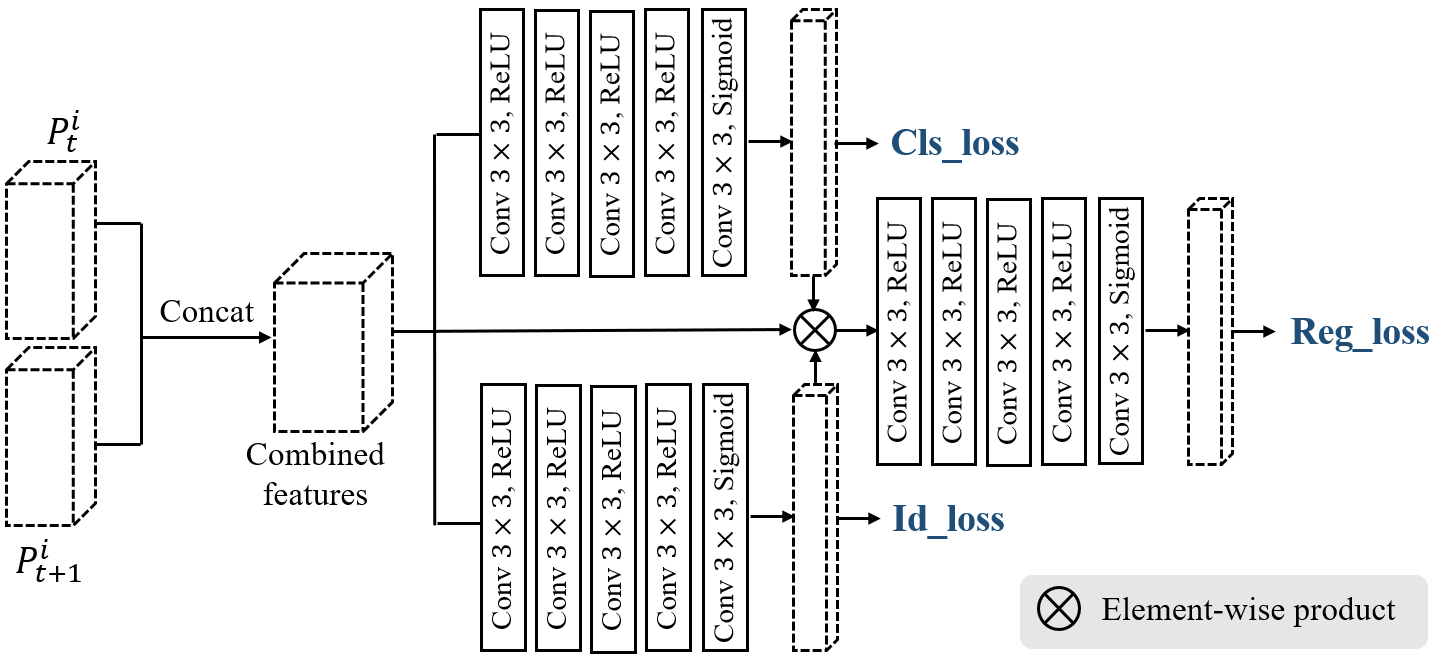
\includegraphics[width=0.90\columnwidth]{figure/figure1.png}
\vspace{-3mm}
\caption{\label{fig:head}\textbf{The detailed architecture of prediction head in CTracker network.} $P_t^i$ and $P_{t+1}^i$ are the multi-scale feautres of two adjacent frames, where $i \in \{2,3,4,5,6\}$.}
\vspace{-3mm}
\end{figure*}

Finally, we gather the above two predictions by multiplication to get the joint attention map. Since the attention map has the same spatial size as the combined features but with only single channel, we first apply broadcasting on the attention map so that they have compatible shapes, then we perform the attention guidance using element-wise product. With the attention-assistant features, we use the paired boxes regression branch with four conv layers to generate paired boxes for objects of interest. All the box pairs generated from the five scales are post-processed with soft-nms \cite{softnms} together. 

\iffalse

\section{Details of Node Chaining\label{section:s_chaining}}

In the Sec. 3.2 of the main text, we introduce that for each unmatched box ${\hat{D}_{t}^{i}}$, it will be retained up to $\sigma$ frames with the constant velocity prediction \cite{wojke2017simple}. This operation is to enhance short-term cross-frame tracking, which is as follows:\\
(1) For each unmatched box pair $(D_{t-1}^{i},\hat{D}_{t}^{i})$, we applying the constant velocity model to predict the box $P_{t+\tau}^{i}$ of the same target in frame $t+\tau$ ($1 <= \tau <= \sigma$) according to $D_{t-1}^{i}$. We use $\mathcal{P}_{t+\tau}$ to represent the set of all the prediction boxes.\\
(2) In frame $t+\tau$, we get the box pair set $\{\mathcal{D}_{t+\tau-1},{\mathcal{\hat{D}}_{t+\tau}}\}$ and $\{\mathcal{D}_{t+\tau},{\mathcal{\hat{D}}_{t+\tau+1}}\}$. $\mathcal{\hat{D}}_{t+\tau}$ and $\mathcal{P}_{t+\tau}$ are matched to $\mathcal{D}_{t+\tau}$ simultaneously. If $P_{t+\tau}^{i}$ is matched, the tracklet which $P_{t+\tau}^{i}$ belongs to is updated by appending the matched box.

\fi

\section{Details of Implementation}

\subsection{Data Augmentation\label{subsection:s_aug}}
In order to construct a robust model for objects with different motion speed, we randomly sample two frames with a temporal interval of no more than 3 frames, then we reverse the order of the two frames with 50\% probability to form a training pair (\textit{i.e.}, $1<=|\delta|<=3$ in Sec. 3.4 of the main text). To further prevent over-fitting, each frame in the pair will be applied with the same data augmentations as follows:\\
(1) Randomly apply some photometric distortions introduced in SSD \cite{liu2016ssd}.\\
(2) Randomly crop a patch of the size determined by multiplying a random factor in the interval [0.3, 0.8] with the image’s shorter side. Note that we only keep those ground truths whose IoMs (Intersection over Min-area) with the cropped patch are greater than 0.2.\\
(3) With 20\% probability, expand the cropped patch using a random factor ranging in [1, 3] by padding with the mean pixel value from ImageNet.\\
(4) Flip the expanded patch randomly and resize it to a square patch with the size equivalent to the half of the original image’s shorter side.

\subsection{Chained-Anchors Setting\label{subsection:s_anchor}}
To determine the scales of Chained-Anchors, we run k-means clustering \cite{yolov2} on all ground truth bounding boxes in the dataset, then we pick five cluster centroids as the scales for Chained-Anchors in different levels of FPN. In our experiments, we use Chained-Anchors of scales $\{38, 86, 112, 156, 328\}$ for $\{P_2, P_3, P_4, P_5, P_6\}$ respectively, and the same ratio of 2.9 is taken for Chained-Anchors of all scales.

\section{Detailed Experiment Results\label{section:s_exp}}

The detailed experiment results of CTracker on MOT16 \cite{milan2016mot16} test dataset and MOT17 test dataset are displayed in Table \ref{tab:mot16_detailed} and Tabel \ref{tab:mot17_detailed}. 

\begin{table}[t!]
\vspace{-10pt}
\renewcommand\arraystretch{1.2}
\centering
\caption{\textbf{Detailed tracking results of CTracker on MOT16 test dataset}.}\label{tab:mot16_detailed}
\vspace{-10pt}
%\footnotesize{
\scriptsize{
\setlength{\tabcolsep}{2.0mm}{
\begin{tabular}{|c|cccccccc|}

\hline

Sequence & MOTA$\uparrow$ & IDF1$\uparrow$ & MOTP$\uparrow$ & MT$\uparrow$ & ML$\downarrow$ & FP$\downarrow$ & FN$\downarrow$ & IDS$\downarrow$\\

\hline
MOT16-01 & 42.0 & 39.3 & 79.9 & 30.4\% & 30.4\% & 713 & 2918 & 77\\
MOT16-03 & 83.6 & 65.5 & 78.3 & 81.1\% & 0.7\% & 5600 & 11024 & 520\\
MOT16-06 & 54.7 & 52.8 & 77.1 & 27.6\% & 24.0\% & 795 & 4158 & 273\\
MOT16-07 & 52.7 & 41.4 & 78.6 & 22.2\% & 13.0\% & 587 & 6884 & 249\\
MOT16-08 & 37.2 & 35.2 & 81.8 & 19.0\% & 33.3\% & 499 & 9824 & 190\\
MOT16-12 & 46.7 & 53.5 & 78.5 & 19.8\% & 37.2\% & 112 & 4250 & 59\\
MOT16-14 & 43.7 & 43.0 & 77.1 & 12.8\% & 32.9\% & 628 & 9247 & 529\\
\hline
Total & 67.6 & 57.2 & 78.4 & 32.9\% & 23.1\% & 8934 & 48305 & 1897\\
\hline
\end{tabular}}}
\end{table}

\begin{table}[t!]
\renewcommand\arraystretch{1.2}
\centering
%\vspace{-30pt}
\caption{\textbf{Detailed tracking results of CTracker on MOT17 test dataset}.}\label{tab:mot17_detailed}
\vspace{-10pt}
%\footnotesize{
\scriptsize{
\setlength{\tabcolsep}{2.0mm}{
\begin{tabular}{|c|cccccccc|}

\hline

Sequence & MOTA$\uparrow$ & IDF1$\uparrow$ & MOTP$\uparrow$ & MT$\uparrow$ & ML$\downarrow$ & FP$\downarrow$ & FN$\downarrow$ & IDS$\downarrow$\\

\hline
MOT17-01 & 51.2 & 44.4 & 78.7 & 25.0\% & 29.2\% & 202 & 2891 & 54\\
MOT17-03 & 84.9 & 66.5 & 77.9 & 83.1\% & 0.7\% & 5133 & 10211 & 479\\
MOT17-06 & 56.1 & 55.2 & 78.2 & 29.7\% & 24.3\% & 516 & 4398 & 261\\
MOT17-07 & 50.2 & 41.0 & 79.3 & 21.7\% & 23.3\% & 424 & 7761 & 228\\
MOT17-08 & 31.6 & 29.6 & 81.2 & 14.5\% & 42.1\% & 405 & 13828 & 212\\
MOT17-12 & 47.0 & 55.7 & 79.2 & 18.7\% & 35.2\% & 91 & 4432 & 69\\
MOT17-14 & 39.5 & 42.7 & 77.4 & 10.4\% & 30.5\% & 657 & 9976 & 540\\
\hline
Total & 66.6 & 57.4 & 78.2 & 32.2\% & 24.2\% & 7428 & 53497 & 1843\\
\hline
\end{tabular}}}
\end{table}



\begin{figure*}[t!]
\centering{}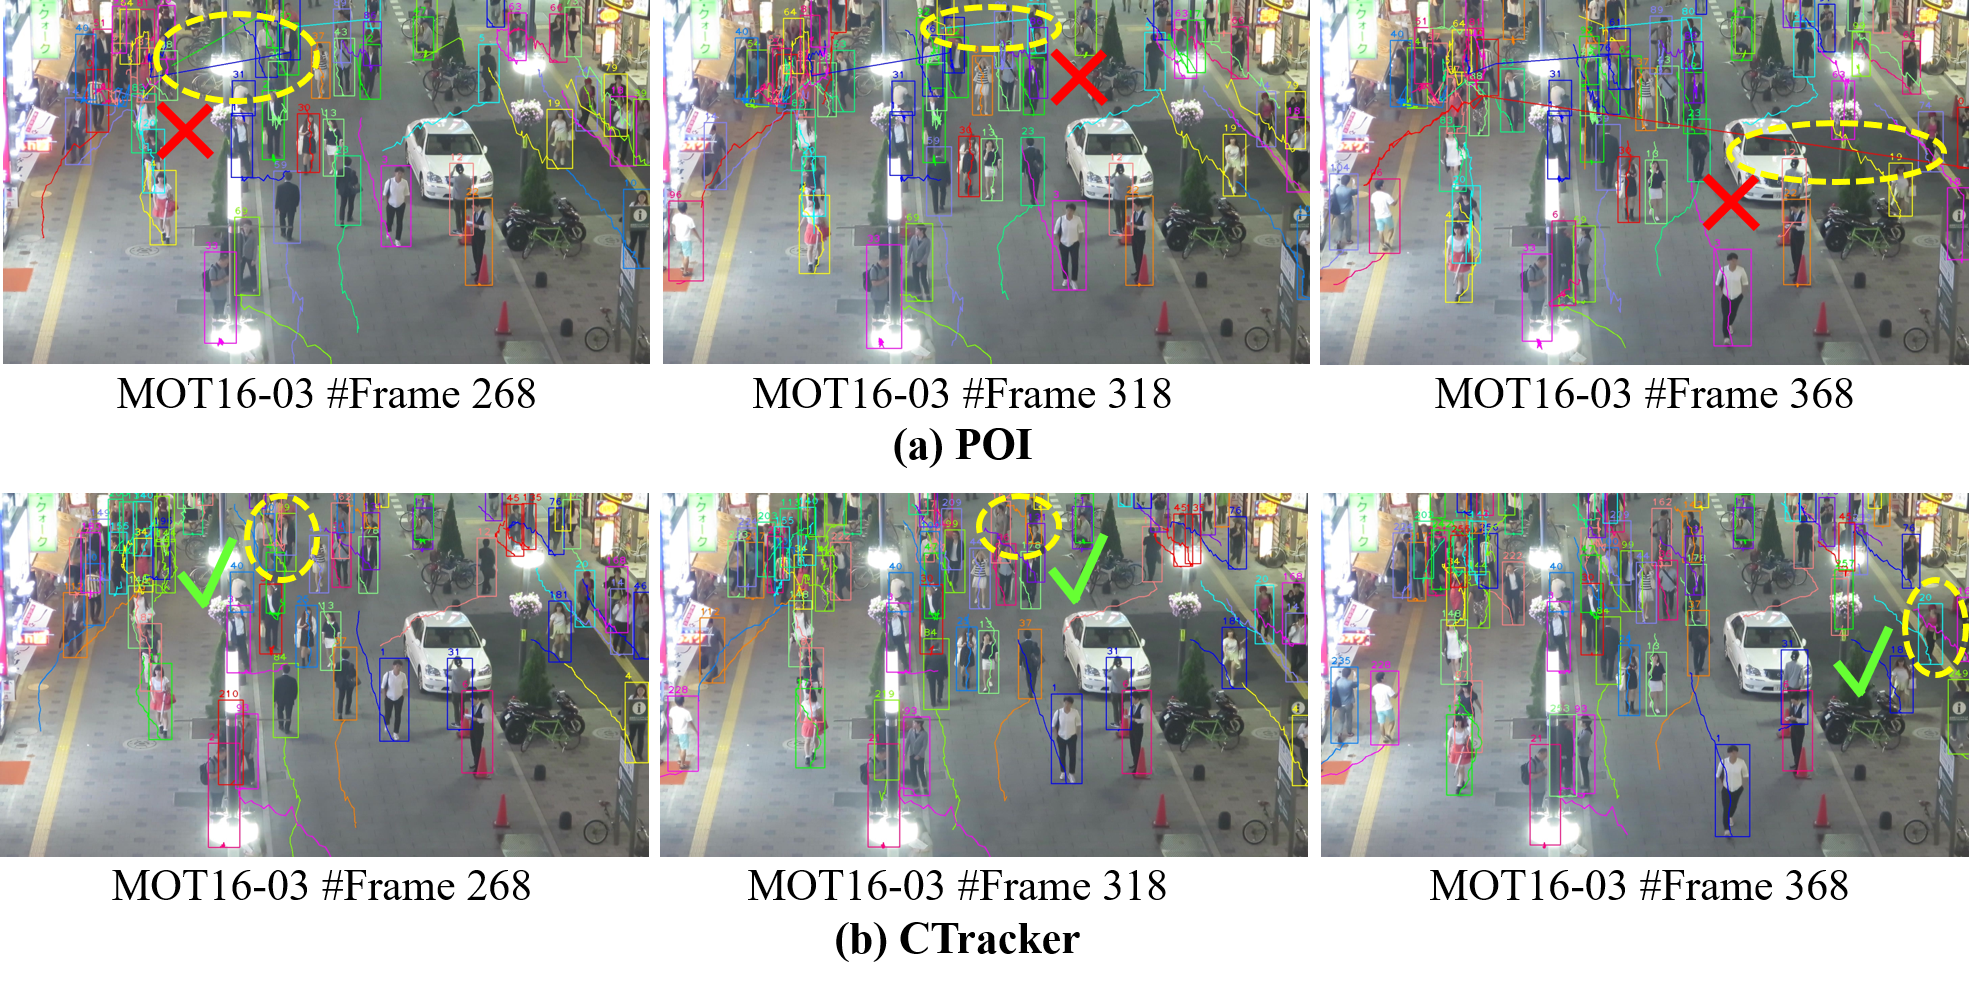
\includegraphics[width=0.98\columnwidth]{figure/poi.png}
\vspace{-5mm}
\caption{\label{fig:poi}\textbf{Qualitative comparison of POI (a) and our CTracker(b).}}
\vspace{-0.04in}
\end{figure*}

\begin{figure*}[t!]
\centering{}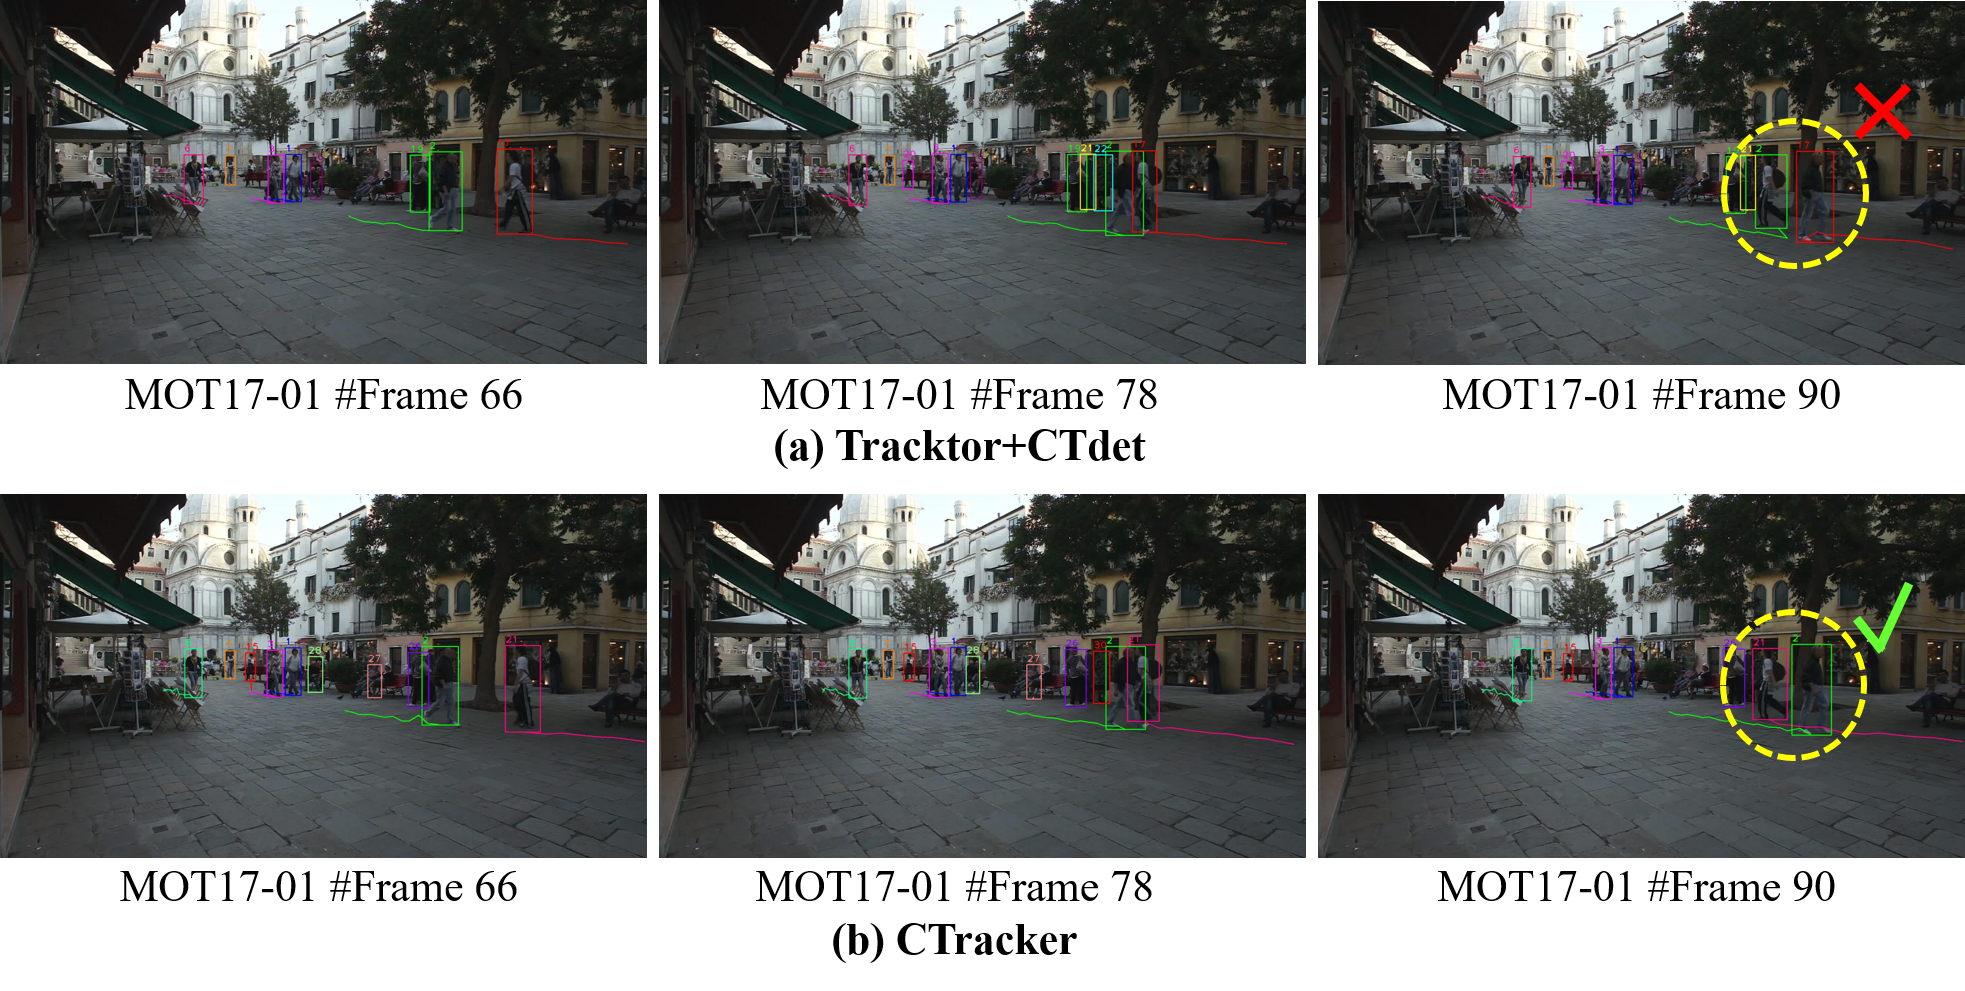
\includegraphics[width=0.98\columnwidth]{figure/tracktor.png}
\vspace{-5mm}
\caption{\label{fig:tracktor}\textbf{Qualitative comparison of Tracktor (a) and our CTracker(b).}}
\vspace{-0.04in}
\end{figure*}

Moreover, we select two representative qualitative cases to compare our CTracker with the private detection online SOTA method POI \cite{yu2016poi} and the public detection online SOTA method Tracktor \cite{bergmann2019tracking}. Fig. \ref{fig:poi} displays the tracking results of POI and our CTracker in sequence MOT16-03. In Fig. \ref{fig:poi}(a), using the POI method, long-term cross-frame tracking drift occurs in several trajectories, which are marked with yellow dotted circles. While in Fig. \ref{fig:poi}(b), using our CTracker method, there is no long-term cross-frame tracking drift in all the trajectories. For simplicity and efficiency, we focus on the short-term tracking based on the Chained-Anchors and abandon using the patch-level ReID features of the detected boxes like POI to enhance long-term cross-frame tracking, which may reduce some trajectory integrity to a certain degree while improve the trajectory accuracy greatly. In Fig. \ref{fig:tracktor}(a), using the Tracktor method with the same detection of our CTracker, there is a ID switch of trajectory 2 and trajectory 17 due to the occlusion, which is marked with a yellow dotted circle. While in Fig. \ref{fig:tracktor}(b), using our CTracker method, the two trajectories representing the same pedestrians are generated correctly due to the accurate box pair association in the CTracker network, which demonstrates the effectiveness of our CTracker in the hard occlusion scene. More complete and clear visualization tracking comparison is displayed in the video attachments.



\section{Appearance Feature Experiment\label{section:s_feature}}



\CRpjl{In the main text, to keep the simplicity and efficiency of our CTracker, we abandon using the patch-level ReID features of the detected boxes like other MOT methods to enhance cross-frame data association. In fact, we conduct a appearance feature experiment though we think that it is not related to our main innovations. In the node chaining module, expect for the IoU affinity, we calculate the appearance similarity by adding in the appearance features (256-dim vector from the feature map before the output convolution in the ID verification branch). On MOT16, MOTA increases from 67.6 to 68.5, IDF1 increases from 57.2 to 61.8, IDS decreases from 1897 to 983. While the tracking speed decreases from 34.4fps to 29.2fps. Therefore, We can get better tracking performance when speed loss is acceptable, demonstrating the good expandability of CTracker.}

% \bibliographystyle{splncs}
% \bibliography{egbib}
\end{document}
